\documentclass[11pt]{article}
\usepackage{CJK}
\usepackage{graphicx}
\usepackage{latexsym,bm}
\usepackage{amsmath}
\usepackage{xcolor}
\usepackage{fancyhdr}
\usepackage{tikz}
\usepackage{colortbl}
\pagestyle{fancy}

\begin{document}
\begin{CJK}{UTF8}{gkai}
%------------------------文章标题---------------------------------------------------------
\title{\textbf{作业一}}
\author{名字\\20122801***}
\date{Oct.17 2012}
\maketitle

\section{问题一}
分析问题...\\
%插入图片
\begin{figure}[!htb]
	\centering
	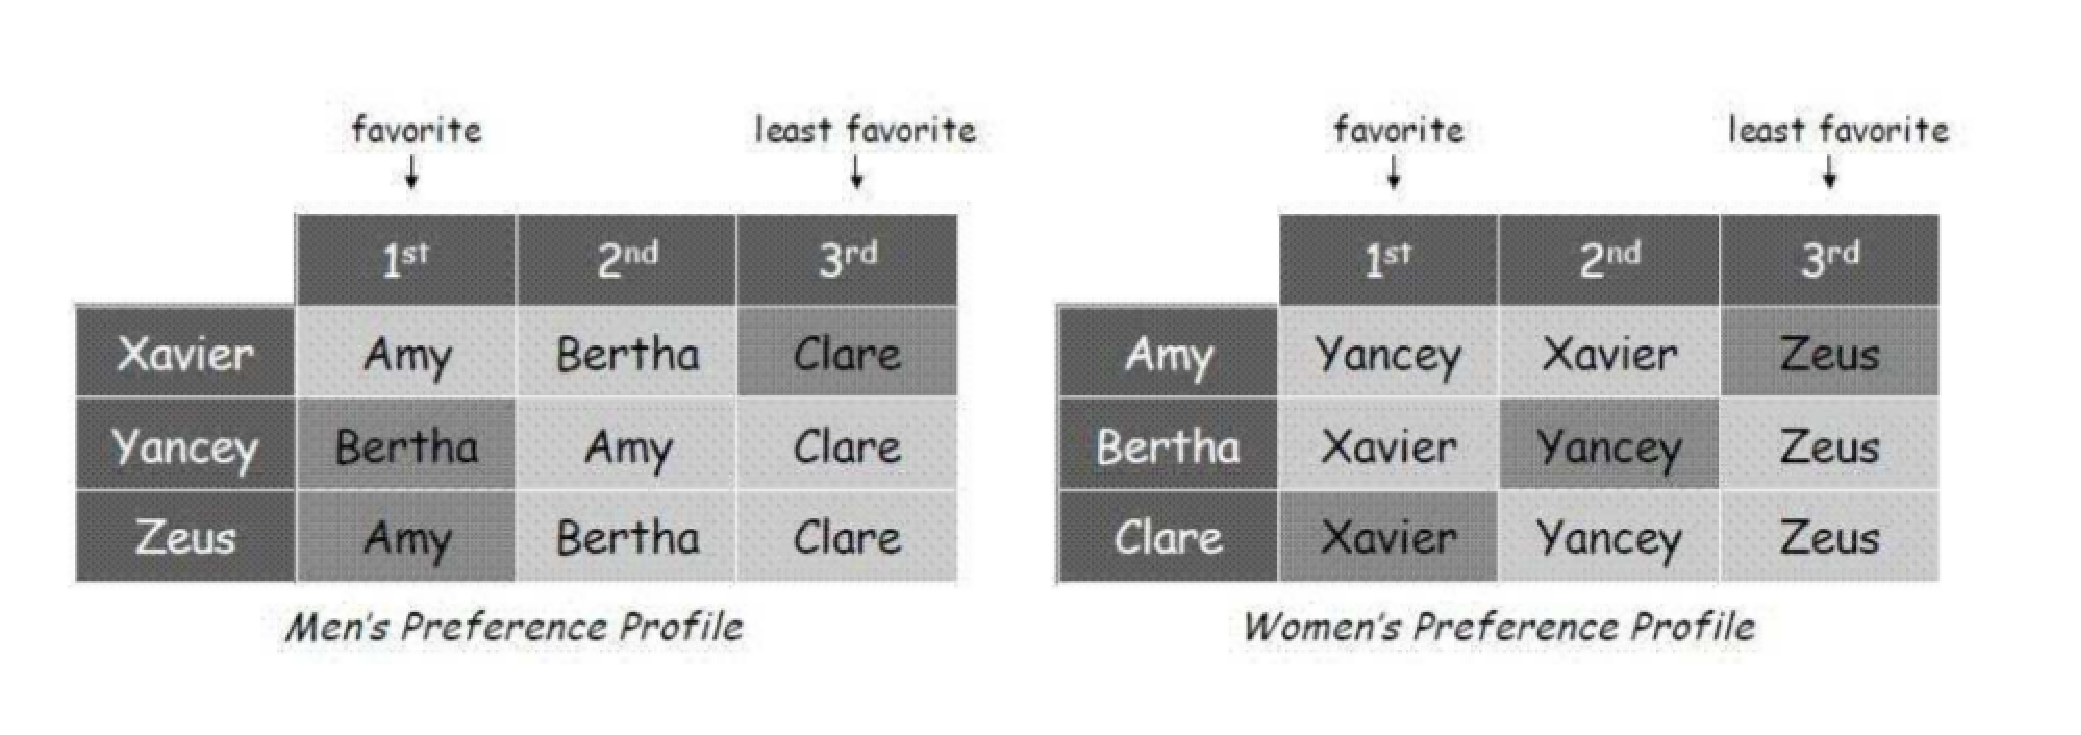
\includegraphics[width=15cm]{1.eps}
	\caption{Preference Table}
\end{figure}

%插入表格
\begin{tabular}{|c|c|c|c|}\hline
{\bf METHODS}{\bf \cellcolor[gray]{.7}  No.}   & $10^5$  & $10^6$ & $10^7$ \\\hline
{\emph MergeSort} & 0.05s    & 0.62s   & 7.07s  \\\hline
{\emph QuickSort} & 0.03s    & 0.40s   & 4.75s  \\\hline
{\emph M\_QuickSort} & 0.04s    & 0.42s   & 5.04s  \\\hline
{\emph MergeSort\_Stack} & 0.06s    & 0.68s   & 7.71s  \\\hline
{\emph QuickSort\_Stack} & 0.04s    & 0.50s   & 5.72s  \\\hline
{\emph M\_QuickSort\_Stack} & 0.04s    & 0.48s   & 5.47s  \\\hline
\end{tabular}\\[5mm]

\end{CJK}
\end{document}
